\chapter{Background}
\label{chap:background}
This chapter provides an overview of the concepts required to understand this thesis. Brief explanations about concepts in Compiler Design are covered here~\cite{aho1977principles}.

\section{Compiler}
\label{sec:compiler}
A translator is a program that converts a program written in one programming language (the source language) into a program in another language (the object or target language). A compiler is a translator, whose source language is a high-level programming language (such as C, C++), and object language is a low-level language such as assembly language or machine language.

The compilation process is divided into 5 phases as shown in Figure \ref{fig:Compiler Phases}.
\begin{figure}
\centering
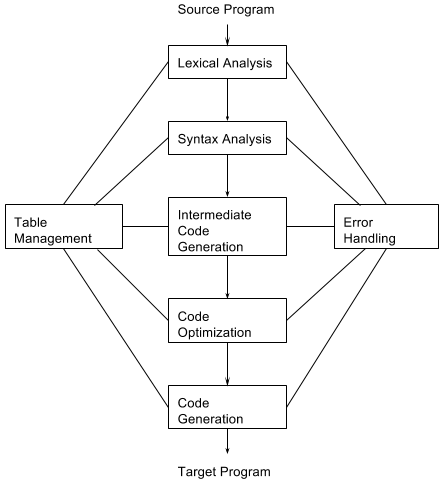
\includegraphics[width=1\textwidth]{CompilerPhases.png}
\caption{Phases of Compiler}
\label{fig:Compiler Phases}
\end{figure}

Following is a brief description of each of the phases of a Compiler:
\begin{enumerate}
\item \textbf{Lexical Analysis:} The first phase of Compiler is called Lexical Analysis. The tool (lexical analyzer or scanner) built for this task, separates the characters of the source language into groups that logically belong together. These groups are called tokens.

The usual tokens are:
\begin{itemize}
\item \textbf{Keywords:} Keywords are the reserved words in a programming language. They have the fixed meaning and cannot be changed by the user. Examples include 'IF', 'WHILE', etc.
\item \textbf{Identifiers:} These are the variables and function names defined by the user in the program, such as 'x', 'sum'.
\item \textbf{Operator Symbols:} They symbolize a specific action and operate on certain values. Examples include '<', '+', etc.
\item \textbf{Punctuation Symbols:} They separates words or phrases (that have meaning to a compiler). Examples include '(', ',', etc.
\end{itemize}
The output of this phase is a stream of tokens, which is passed to the next phase of Compiler.

\item \textbf{Syntax Analysis:} The syntax analyzer or parser groups tokens together into syntactic structures. If A*B+C is a string (containing 5 tokens), then it can be considered as (A*B)+C or as A*(B+C), depending on the language definition. The syntactic structure determines how these tokens are to be grouped together into larger structures called syntactic categories such as: \textbf{expressions} - sequences of operator and operands (constants and identifiers) or \textbf{statements} - multiple expressions can be combined to form statements.

The syntactic structure can be represented as a tree, known as a parse tree. Tokens appear on the leaves of this tree and the interior nodes of the tree represent strings of tokens that logically belong together.
\begin{example}
The three tokens representing 'A+B' can be grouped into an expression. The parse tree for 'A+B' can be represented as in Figure \ref{fig:SyntaxTree}.
\begin{figure}
\centering
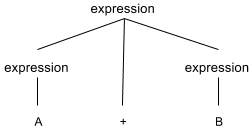
\includegraphics[width=0.5\textwidth]{SyntaxTree.png}
\caption{Parse Tree for A+B}
\label{fig:SyntaxTree}
\end{figure}
\end{example}

\item \textbf{Intermediate Code Generation:} The intermediate code generator uses the structure produced by the syntax analyzer to create a stream of simple instructions. These instructions can be in the form of "Macros".

\textbf{Macros} are small functions which can be converted into assembly language code.
\begin{example}
For addition, a macro can be defined as:
\begin{minted}{C}
MACRO   ADD2    X,Y
        LOAD    Y
        ADD     X
        STORE   Y
ENDMACRO
\end{minted}
For A+B, this macro can be used as:
\begin{minted}{C}
LOAD    B
ADD     A
STORE   B
\end{minted}
\end{example}

\item \textbf{Code Optimization:} This phase is used to improve the intermediate code so that the final object program runs faster and/or takes less space. Its output is another intermediate code program which is an improved version of the previous one.
\begin{example}
Suppose we have the following code snippet:
\begin{minted}{Java}
while(j<=10)
{
    i = 2;
    j = j + i;
}
\end{minted}

Here, the assignment i = 2 is executed in every iteration of the loop. But, the value of i remains constant in all iterations and is not changed in the loop. So, this assignment statement can be placed outside the loop to optimize the code such as
\begin{minted}{Java}
i = 2;
while(j<=10)
{
    j = j + i;
}
\end{minted}
\end{example}

\item \textbf{Code Generation:} This is the final phase of Compiler. It produces the object code by deciding on the memory locations for data, selecting code to access each datum, and selecting the registers in which each computation is to be done.
\begin{example}
For the instruction "A+B", code can be generated as:
\begin{minted}{C}
MOV A, R0
ADD B, R0
\end{minted}
\end{example}

\item \textbf{Table Management:} Table Management or book-keeping keeps track of the names used by the program and records essential information about each. An example of information is the type (integer, real) of a variable. For storing such information a data structure known as a symbol table is used.

\item \textbf{Error Handling:} The error handler warns the programmer about the flaws in the source program, by issuing a diagnostic and adjusting the information being passed from phase to phase, so that compilation can proceed till the last phase.
\end{enumerate}

\subsection{Some Terminology}
\label{subsec:Terminology}
Some terms related to the parsing phase of Compiler have been used in this thesis. A brief description of these terms is given below:
\begin{itemize} %add ref{https://en.wikipedia.org/wiki/Formal_grammar}
\item \textbf{Alphabet:} The set of symbols used in a programming language is called the alphabet of that programming language. Eg: \{a,b\}.
\item \textbf{Language:} Any set of strings formed from some specific alphabet. Eg: L = \{\{$\epsilon$, a, b, aa, bb, ab, ba\} | \{a,b\} $\in$ alphabet\}.
\item \textbf{Kleene Closure:} It is a unary operation defined as follows: if V is a set of symbols or characters, then V* (kleene closure) is the set of all strings over symbols in V, including the empty string $\epsilon$.
\item \textbf{Grammar:} A grammar is a set of production rules, to form strings from a language's alphabet. A grammar checks the validity of strings, by checking their syntactic correctness.

A grammar G = (N, $\Sigma$, P, S) consists of the following components:
\begin{itemize}
\item A finite set \textbf{N} of non-terminals (synonym for syntactic categories), that is disjoint with the strings formed from G.
\item A finite set \textbf{$\Sigma$} of terminals (synonym for tokens) that is disjoint from N.
\item A finite set \textbf{P} of production rules, each rule of the form \\
 $(\Sigma \cup N)^{*} N (\Sigma \cup N)^{*} \rightarrow (\Sigma \cup N)^{*}$ \\
where * is the Kleene closure and $\cup$ denotes set union.
\item The symbol \textbf{S}, where S $\in$ N is the start symbol.
\end{itemize}

\begin{example}
The grammar G, where N = $\left \{S, B\right \}$, $\Sigma = \left \{a, b, c\right \}$, S is the start symbol, and P consists of the following production rules:
\item $S \rightarrow aBSc$
\item $S \rightarrow abc$
\item $Ba \rightarrow aB$
\item $Bb \rightarrow bb$
\end{example}

\item \textbf{Context-free Grammar:} A context-free grammar(CFG) is a grammar in which the left-hand side of each production rule consists of only a single non-terminal symbol.
\begin{example}
\label{ex:CFG}
The grammar with N = $\left \{S\right \}$, $\Sigma=\left \{a,b\right \}$, S the start symbol, and the following production rules, P:
\item $S \rightarrow aSb$
\item $S \rightarrow ab$
\end{example}

\item \textbf{Derivation:} A derivation replaces a non-terminal on the LHS of a production with its respective RHS.
\begin{example}
One of the strings, which can be derived from the grammar in example \ref{ex:CFG}, by the following steps:

$S \Rightarrow aSb \Rightarrow aaSbb \Rightarrow aaabbb$
\end{example}
If the leftmost non-terminal is always expanded in the derivation, to acquire the string, then it is a leftmost derivation. Similarly if  the rightmost non-terminal is always expanded, then it is a rightmost derivation.
\begin{example}
Suppose the grammar is:
\begin{eqnarray*}
E&\rightarrow& T\ E'\\
E'&\rightarrow& +\ E \\
  & \mid& \epsilon\\
T&\rightarrow&0
\end{eqnarray*}

then, the following is the leftmost derivation

$E \Rightarrow TE' \Rightarrow 0E' \Rightarrow 0+E \Rightarrow 0+TE' \Rightarrow 0+0E' \Rightarrow 0+0$

and the rightmost derivation can be

$E \Rightarrow TE' \Rightarrow T+E \Rightarrow T+TE' \Rightarrow T+T \Rightarrow T+0 \Rightarrow 0+0$
\end{example}

\item \textbf{Sentential Form:} Let G = (N, $\Sigma$, P, S) be a CFG, and $\alpha\in(N\cup\Sigma)^*$. If $S\overset{*}{\Rightarrow}\alpha$ (where $\overset{*}{\Rightarrow}$ means derivation in zero or more steps), then $\alpha$ is the sentential form.

If $S\underset{lm}{\Rightarrow}\alpha$ (leftmost derivation), then $\alpha$ is a left-sentential form and if $S\underset{rm}{\Rightarrow}\alpha$ (rightmost derivation), then $\alpha$ is a right-sentential form.
%add ref http://www.univ-orleans.fr/lifo/Members/Mirian.Halfeld/Cours/TLComp/res1-CG.pdf
\begin{example}
Consider the example \ref{ex:CFG}. Each of \{S, aSb, aaSbb, aaabbb\}, derived from the set of production rules, is a sentential form.
\end{example}

\item \textbf{Lookahead:} Some parsing algorithms use a technique of looking ahead certain tokens in order to decide which rule to use. The maximum number of tokens that a parser can use to decide which rule it should use, is known as lookahead. % add ref https://en.wikipedia.org/wiki/Lookahead

\item \textbf{Handle:} A handle of a string is a substring that matches the right side of a production and whose reduction to the non-terminal on the left side of the production represents one step along the reverse of a rightmost derivation. 

A handle of a right-sentential form $\gamma$ is a production $A \rightarrow \beta$ and a position of $\gamma$ where the string $\beta$ may be found and replaced by A to produce the previous right-sentential form in a rightmost derivation of $\gamma$. That is, if $S\overset{*}{\Rightarrow} \alpha Aw \Rightarrow \alpha \beta w$, then $A \rightarrow \beta$ in the position following $\alpha$ is a handle of $\alpha \beta w$. the string w to the right of the handle contains only terminal symbols.
% ullman

\item \textbf{DFA:} Deterministic Finite Automaton is a finite state machine that accepts or rejects finite strings of symbols and only produces a unique computation (or run) of the automaton for each input string.
%https://en.wikipedia.org/wiki/Deterministic_finite_automaton

A DFA A = (Q, $\Sigma$, $\delta$, q_0, F) consists of:
\begin{enumerate}
\item A finite set of states, denoted by Q.
\item A finite set of input symbols, denoted by $\Sigma$.
\item A transition function, denoted by $\delta$, that takes as arguments a state and an input symbol and returns a state. Eg: If q is a state and a i an input symbol, then $\delta(q,a)$ is that state p such that there is an arc labeled a from q to p.
\item A start state, denoted by q_0. It is one of the states in Q.
\item A set of final or accepting states F. The set F is a subset of Q.
\end{enumerate}
%book: toc hopcroft

\end{itemize}

\subsection{Parsing Phase of Compiler}
\label{subsec:Parsing Phase}
Parsing is the second phase of Compiler. It is performed after Lexical Analysis. A sequence of tokens (output of the lexical analyzer), is passed to parsing phase as input. The parser then checks whether the input string is syntactically correct or not. For this task, a CFG is used to define the syntax of a programming language. A parsing table is constructed, using the CFG, which is used to parse the input strings.

There are various parsing techniques which are discussed in the later parts of this chapter. The following section briefly describes FIRST and FOLLOW set, which is necessary for constructing parsing tables.

\subsubsection{Preliminaries}
\label{ssubsec:preliminary}

\begin{itemize}
\item \textbf{FIRST:} If $\alpha$ is any string of grammar symbols, then FIRST$(\alpha)$ is the set of all terminals, that appear in the beginning of strings derived from $\alpha$. If $\alpha\overset{*}{\Rightarrow}\epsilon$, then $\epsilon$ is also in FIRST($\alpha$).

To compute FIRST(X) for all grammar symbols X, apply the following rules until no more terminals or $\epsilon$ can be added to any FIRST set.
\begin{enumerate}
\item If X is a terminal, then FIRST(X) is {X}.
\item If X is a non-terminal and X $\to$ a$\alpha$ is a production, then add a to FIRST(X). If X $\to$ $\epsilon$ is a production, then add $\epsilon$ to FIRST(X).
\item If X $\to$ Y_1Y_2....Y_k is a production, then for all i such that all of Y_1,....,Y_{i-1} are non-terminals and FIRST(Y_j) contains $\epsilon$ for j = 1, 2, ...., i-1 (i.e Y_1Y_2....Y_{i-1} $\overset{*}{\Rightarrow}\ \epsilon$), add every non-$\epsilon$ symbol in FIRST(Y_i) to FIRST(X). If $\epsilon$ is in FIRST(Y_j) for all j = 1, 2, ....., k, then add $\epsilon$ to FIRST(X).
\end{enumerate}

\begin{example}
\label{ex:First}
Suppose the grammar is
\begin{eqnarray*}
E &\to& T E'\\
E'&\to& \epsilon | + E\\
T &\to& 0 | 1\\
\end{eqnarray*}
Then

FIRST[E] = \{1, 0\}

FIRST[E'] = \{+, $\epsilon$\}

FIRST[T] = \{1, 0\}
\end{example}

\item \textbf{FOLLOW:} FOLLOW(A), for non-terminal A, is the set of terminals, that can appear immediately to the right of A, in some sentential form. That is, $S\overset{*}{\Rightarrow}\alpha Aa\beta$ for some $\alpha$ and $\beta$. If A is the rightmost symbol in some sentential form, then we add \$ to FOLLOW(A).
\begin{enumerate}
\item \$ is in FOLLOW(S), where S is the start symbol. %
\item If there is a production $A\to\alpha B\beta$, $\beta\neq\epsilon$, then everything in FIRST($\beta$) but $\epsilon$ is in FOLLOW(B).
\item If there is a production $A\to\alpha B$, or a production $A\to\alpha B\beta$ where FIRST($\beta$) contains $\epsilon$ (i.e., $\beta\overset{*}{\Rightarrow}\epsilon$), then everything in FOLLOW(A) is in FOLLOW(B).
\end{enumerate}

\begin{example}
\label{ex:Follow}
For the grammar used in example \ref{ex:First}

FOLLOW[T] = \{\$, +\}

FOLLOW[E] = \{\$\}

FOLLOW[E'] = \{\$\}
\end{example}
\end{itemize}

\subsubsection{LL Parsing}
\label{ssubsec:LL Parsing}
It is a top-down parsing technique. The first L in LL(1) stands for parsing the input from Left to right and the second L for performing Leftmost derivation of the input string (1 is the number of lookaheads). Because of this lookahead, the parser is categorised as a predictive parser. To parse an input string, it starts with the root and works down to the leaves. Here, start symbol is the root of the parse tree and the sequence of terminals, in the input string, forms the leaves of the tree. Every parse tree represents a string generated by the grammar.
\begin{example}
If the grammar is:

S $\to$ cAd

A $\to$ a | ab

The parse tree for the string 'cad' is represented in figure \ref{fig:Parse Tree}.
\begin{figure}
\centering
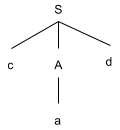
\includegraphics[width=0.3\textwidth]{ParseTree.png}
\caption{Parse Tree for string cad}
\label{fig:Parse Tree}
\end{figure}

\end{example}

There are several difficulties with this parsing technique. One of them is Left-recursion. A grammar G is said to be left-recursive if it has a non-terminal A such that there is a derivation $A\overset{+}{\Rightarrow}A\alpha$ ($\overset{+}{\Rightarrow}$ represents derivation in 1 or more steps) for some $\alpha$. A left-recursive grammar can cause the top-down parser to go into an infinite loop. Hence such grammars are not LL(1) and are not supported by LL Parsing.

Another issue with this parsing technique is left-factoring. Suppose if we have a production such as: A $\to$ abc | ab, then on seeing a, we could not tell, which production to choose, in order to expand the statement. For solving this problem, left-factoring is performed on the grammar. It is the process of factoring out the common prefixes of alternates. The following example explains the procedure of left-factoring:
\begin{example}
If A$\to$ $\alpha\beta$ | $\alpha\gamma$ are two productions in the grammar, then after left-factoring, the production rules are of the form:

A $\to$ $\alpha A'$

A' $\to$ $\beta$ | $\gamma$
\end{example}
To parse an input string using LL parsing, LL Parsing table is required. Following is a brief description of a LL parsing table and the calculation of LL parsing moves.

\paragraph{LL Parsing Table}\mbox{}\\
\label{para: LL Paring Table}
It is a two-dimensional array M[A, b], where A is a non-terminal and b is a terminal or \$. The entries in the LL parsing table are filled by using FIRST and FOLLOW sets. An input string is parsed by using this table.

Algorithm \ref{algo:LL Parsing Table} described below, can be used to construct the LL parsing table for a grammar G.
\begin{algorithm}
\caption{Construction of LL Parsing Table}
\label{algo:LL Parsing Table}

\begin{algorithmic}[1]
\Require Grammar G.
\Ensure Parsing Table M.
\State For each production A $\to$ $\alpha$ of the grammar, do steps 2 and 3.
\State For each terminal a in FIRST($\alpha$), add A $\to$ $\alpha$ to M[A, a].
\State If $\epsilon$ is in FIRST($\alpha$), add A $\to$ $\alpha$ to M[A, b] for each terminal b in FOLLOW(A). If $\epsilon$ is in FIRST($\alpha$) and \$ is in FOLLOW(A), add A $\to$ $\alpha$ to M[A, \$].
\State Make each undefined entry of M error.
\end{algorithmic}
\end{algorithm}

The undefined entries are usually left blank, instead of writing error in them.
\begin{example}
\label{ex:LL table}
For the grammar used in example \ref{ex:First}, LL Parsing table can be filled using the above algorithm as:
\begin{center}
\begin{tabular}{ |c|c|c|c|c| } 
 \hline
  & \textbf{0} & \textbf{1} & \textbf{+} & \textbf{\$} \\
 \hline
 \textbf{T} & T $\to$ 0 & T $\to$ 1 &  &  \\
 \hline
 \textbf{E} & E $\to$ T E' & E $\to$ T E' &  &  \\
 \hline
 \textbf{E'} &  &  & E' $\to$ + E & E' $\to$ $\epsilon$ \\
 \hline
\end{tabular}
\end{center}
\end{example}
A grammar is said to be LL(1) if there are no multiply-defined entries in its parsing table. Left-recursive grammars are not LL(1). Also, left-factoring must be performed on grammars if required, otherwise, they may result in multiple entries in a cell of LL parsing table.

\paragraph{LL Parsing Moves}\mbox{}\\
\label{para: LL Parsing Moves}
The parser has an input, a stack, a parsing table, and an output as shown in figure \ref{fig:LL Parser}.
\begin{figure}
\centering
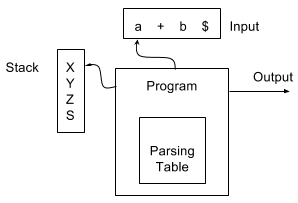
\includegraphics[width=0.5\textwidth]{LLParsingModel.png}
\caption{Model of a predictive parser}
\label{fig:LL Parser}
\end{figure}
The input contains the string to be parsed, followed by \$, the right endmarker. The stack contains a sequence of grammar symbols, preceded by \$ (the bottom-of-stack marker). The contents of the stack, in each step, show the leftmost derivation on the input string. Output shows the action done in each step.

If X is the symbol on top of the stack and a is the current input symbol, then following are the rules that determine the action of the parser.
\begin{enumerate}
\item If X = a = \$, the parser halts and announces successful completion of parsing.
\item If X = a $\neq$ \$, the parser pops X off the stack and advances the input pointer to the next input symbol.
\item If X is a nonterminal, the program consults entry M[X, a] of the parsing table M. If M[X, a] = {X $\to$ UVW}, the parser replaces X on top of the stack by WVU (with U on top). If M[X, a] = error, the parser calls an error recovery routine.
\end{enumerate}

The following example shows the parsing of an input string by applying the above rules. Initially, the stack contains the start symbol of the grammar preceded by \$.
\begin{example}
\label{ex:LL moves}
For the same grammar used in example \ref{ex:First}, if the input string is "0 + 1", then the parsing moves are:
\begin{center}
\begin{tabular}{ |>{\raggedright\arraybackslash$}p{3cm}<{$}|>{\raggedleft\arraybackslash$}p{3cm}<{$}|c| } 
 \hline
 \textbf{STACK} & \textbf{INPUT} & \textbf{OUTPUT} \\
 \hline
 \$ E & 0 + 1 \$ & \\
 \$ E' T & 0 + 1 \$ & E $\to$ T E' \\ 
 \$ E' 0 & 0 + 1 \$ & T $\to$ 0 \\
 \$ E' & + 1 \$ & \\
 \$ E + & + 1 \$ & E' $\to$ + E \\
 \$ E & 1 \$ & \\  
 \$ E' T & 1 \$ & E $\to$ T E' \\
 \$ E' 1 & 1 \$ & T $\to$ 1 \\
 \$ E' & \$ & \\
 \$ & \$ & E' $\to \epsilon$ \\
 \hline
\end{tabular}
\end{center}
\end{example}

\subsubsection{SLR Parsing}
\label{ssubsec:SLR Parsing}
It is one of the LR parsing techniques. It is a bottom-up parsing method. As the name implies, LR parsers scan the input from left-to-right and construct a rightmost derivation in reverse. SLR stands for Simple LR Parsing. K is usually 1 for this parsing. It is the easiest to implement, but may fail to produce a table for certain grammars.

This parsing works on left-recursive grammars, but it is necessary to perform left-factoring if required.

To construct the SLR parsing table, the canonical collection of SLR items are calculated. In later parts of this section, a brief discussion about canonical sets, SLR parsing table and moves is given.

\paragraph{Canonical Collection of SLR Items}\mbox{}\\
\label{para:Canonical Set}
To construct the parsing table, a DFA from the grammar is constructed. The DFA recognizes viable prefixes of the grammar, that is, prefixes of right-sentential forms that do not contain any symbols to the right of the handle.

SLR item of a grammar G is defined as a production of G with a dot at some position on the right side, which indicates how much of a production we have seen at a given point in the parsing process. Thus, production $A\rightarrow XYZ$ generates the four items:

$A\rightarrow .XYZ$

$A\rightarrow X.YZ$

$A\rightarrow XY.Z$

$A\rightarrow XYZ.$

and the production "$A\rightarrow \epsilon$" generates only one item, "$A\rightarrow.$" . As an example, the second item in the above productions, would indicate that we have just seen on the input, a string derivable from X and that we next expect to see a string derivable from YZ. These items are grouped together as itemsets, which are further grouped to form a Canonical SLR collection. To construct this collection we need to define an augmented grammar and two functions - CLOSURE and GOTO.

\begin{itemize}
\item \textbf{Augmented Grammar:} If G is a grammar with start symbol S, then G', the augmented grammar for G, is G with a new start symbol S' and production $S'\rightarrow S$. This new starting production is used to indicate to the parser when it should stop parsing and announce acceptance of the input. This would occur when the parser was about to reduce by $S'\rightarrow S$.

\item \textbf{CLOSURE:} If I is a set of items for a grammar G, then the set of items CLOSURE(I) is constructed from I by the rules:
\begin{enumerate}
\item Every item in I is in CLOSURE(I).
\item If $A\rightarrow\alpha.B\beta$ is in CLOSURE(I) and $B\rightarrow\gamma$ is a production, then add the item $B\rightarrow.\gamma$ to I, if it is not already there.
\end{enumerate}

Following example illustrate the CLOSURE function:
\begin{example}
\label{ex:Closure}
Suppose the augmented grammar is:

$E''\rightarrow E$

$E\rightarrow TE'$

$E'\rightarrow \epsilon | +E$

$T\rightarrow 0 | 1$

If I is the set of one item {[$E''\rightarrow .E$]}, then CLOSURE(I) contains the items

E'' $\rightarrow$ .E

E $\rightarrow$ .TE'

T $\rightarrow$ .1

T $\rightarrow$ .0
\end{example}

\item \textbf{GOTO:} GOTO(I, X), where I is a set of items and X is a grammar symbol, is the closure of the set of all items $[A\rightarrow\alpha X.\beta]$ such that $[A\rightarrow\alpha.X\beta]$ is in I.
Following example illustrates the calculation of GOTO function:
\begin{example}
For the augmented grammar used in example \ref{ex:Closure}, if I is the set of items \{$[E''\rightarrow.E]$, $[E\rightarrow .TE']$, $[T\rightarrow.0]$, $[T\rightarrow.1]$\}, then GOTO(I, T) consists of:

E $\to$ T.E'

E' $\to$ .
    
E' $\to$ .+E
\end{example}
\end{itemize}

The algorithm \ref{algo:SLR Canonical Set} is used to construct C, the canonical collection of sets of LR(0) items for an augmented grammar G'.
\begin{algorithm}
\caption{Canonical collection of sets of SLR items Construction}
\label{algo:SLR Canonical Set}

\begin{algorithmic}[1]
\State C = {CLOSURE(${S'\rightarrow.S}$)}
\Repeat
\For{each set of items I in C and each grammar symbol X such that GOTO(I, X) is not empty and is not in C}
\State add GOTO(I, X) to C
\EndFor
\Until{no more sets of items can be added to C}
\end{algorithmic}
\end{algorithm}

Following example illustrates the construction of collection of sets of LR(0) items:

\begin{example}
\label{ex:SLR set}
For the augmented grammar used in example \ref{ex:Closure}, SLR Canonical set is
\begin{itemize}
\item[I0:] T $\to$ .1 \\
           T $\to$ .0 \\
           E'' $\to$ .E \\
           E $\to$ .TE'
\item[I1:] E $\to$ T.E' \\
           E' $\to$ . \\
           E' $\to$ .+E
\item[I2:] T $\to$ 1.
\item[I3:] T $\to$ 0.
\item[I4:] E'' $\to$ E.
\item[I5:] T $\to$ .1 \\
           E $\to$ .TE' \\
           E' $\to$ +.E \\
           T $\to$ .0
\item[I6:] E $\to$ TE'.
\item[I7:] E' $\to$ +E.
\end{itemize}
\end{example}

\paragraph{SLR Parsing Table}\mbox{}\\
\label{para:SLR Parsing Table}
This table is divided into two parts - Action and Goto. Algorithm \ref{algo:SLR Parsing Table} shows the construction of 
SLR parsing action and goto functions from the DFA that recognizes viable prefixes. Each entry in the table determines whether to shift the input symbol on the stack or to reduce a string of symbols on top of stack by a single symbol using the productions of grammar.

\begin{algorithm}
\caption{Construction of SLR Parsing Table}
\label{algo:SLR Parsing Table}

\begin{algorithmic}[1]
\Require C, the canonical collection of sets of items for an augmented grammar G'.
\Ensure If possible, an LR parsing table consisting of a parsing action function ACTION and a goto function GOTO.
\Statex Let C = {I_0, I_1,...., I_n}. The states of the parser are 0, 1,..., n, state i being constructed from I_i. The parsing actions for state i are determined as follows:
\If{$[A\rightarrow\alpha.a\beta]$ is in I_i and GOTO(I_i, a) = I_j} \label{line:shift}
\State set ACTION[i, a] to "shift j". Here a is a terminal.
\EndIf
\If{$[A\rightarrow\alpha.]$ is in I_i}
\State set ACTION[i, a] to "reduce $A\rightarrow\alpha$" for all a in FOLLOW(A).
\EndIf
\If{$[S'\rightarrow\alpha S.]$ is in I_i}
\State set ACTION[i, \$] to "accept".
\EndIf
\Statex The goto transitions for state i are constructed using the rule:
\If{GOTO(I_i, A) = I_j}
\State GOTO[i, A] = j.
\EndIf  \label{line:goto}
\State All entries not defined by rules \ref{line:shift} through \ref{line:goto} are made "error".
\State The initial state of the parser is the one constructed from the set of items containing [S'$\rightarrow$ .S].
\end{algorithmic}
\end{algorithm}

Following example shows the SLR parsing table for an augmented grammar.
\begin{example}
\label{ex:SLR table}
For the grammar used in example \ref{ex:Closure}, SLR Parsing table is
\begin{center}
\begin{tabular}{ |c|c|c|c|c|c|c|c| }
 \hline
 \textbf{STATE} & \multicolumn{4}{c}{\textbf{ACTION}} & \multicolumn{3}{|c|}{\textbf{GOTO}}\\
 \hline
  & \textbf{0} & \textbf{1} & \textbf{+} & \textbf{\$} & \textbf{T} & \textbf{E} & \textbf{E'}\\
 \hline
 \textbf{0} & s3 & s2 &  &  & 1 & 4 & \\
 \hline
 \textbf{1} &  &  & s5 & r4 &  &  & 6\\
 \hline
 \textbf{3} &  &  & r1 & r1 &  &  & \\
 \hline
 \textbf{4} &  &  &  & accept &  &  & \\
 \hline
 \textbf{5} & s3 & s2 &  &  & 1 & 7 & \\
 \hline
 \textbf{6} &  &  &  & r3 &  &  & \\
 \hline
 \textbf{7} &  &  &  & r5 &  &  & \\
 \hline
\end{tabular}
\end{center}
Blank entries are the "error" entries.
\end{example}

\paragraph{SLR Parsing Moves}\mbox{}\\
\label{para: SLR Parsing Moves}
An LR parser consists of two parts - a driver routine and a parsing table. The driver routine is the same for all LR parsers, but the parsing table changes from one parser to another. Figure \ref{fig:LR Parser} shows the model of LR Parsers.
\begin{figure}
\centering
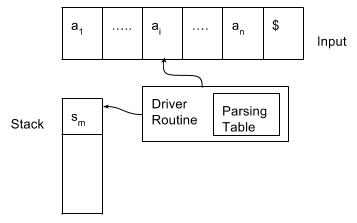
\includegraphics[width=0.5\textwidth]{SLRParsingModel.png}
\caption{Model of a SLR parser}
\label{fig:LR Parser}
\end{figure}

The input is read from left to right, one symbol at a time. The stack contains a string of the form s_0X_1s_1X_2s_2....X_ms_m, where s_m is on top. Each X_i is a grammar symbol and each s_i is the state.

The entry ACTION[s_m, a_i], where s_m is the state on top of stack and a_i is the current input symbol, can have one of four values:
\begin{enumerate}
\item shift s.
\item reduce $A\rightarrow\beta$.
\item accept.
\item error.
\end{enumerate}
The function GOTO takes a state and grammar symbol as arguments and produces a state.

A configuration of an LR parser is a pair whose first component is the stack contents and whose second component is the unexpected input:

(s_0 X_1 s_1 X_2 s_2 ... X_m s_m, a_i a_{i+1} ... a_n \$)

The configurations resulting after each of the four types of move, on consulting the parsing action table entry ACTION[s_m, a_i], are as follows:
\begin{enumerate}
\item If ACTION[s_m, a_i] = shift s, the parser executes a shift move, entering the configuration

(s_0 X_1 s_1 X_2 s_2 ... X_m s_m a_i s, a_{i+1} ... a_n \$)

Here the parser has shifted the current input symbol a_i and the next state s = GOTO[s_m, a_i] onto the stack. a_{i+1} becomes the new current input symbol.
\item If ACTION[s_m, a_i] = reduce $A\rightarrow\beta$, then the parser executes a reduce move, entering the configuration

(s_0 X_1 s_1 X_2 s_2 ... X_{m-r} s_{m-r} A s, a_i a_{i+1} ... a_n \$)

where s = GOTO[s_{m-r}, A] and r is the length of $\beta$, the right side of the production. Here the parser first popped 2r symbols off the stack (r state symbols and r grammar symbols), exposing state s_{m-r}. The parser then pushed both A, the left side of the production, and s, the entry for ACTION[s_{m-r}, A], onto the stack. The current input symbol is not changed in a reduce move. For the LR parsers we shall construct, X_{m-r+1} ... X_m, the sequence of grammar symbols popped off the stack, will always match $\beta$, the right side of the reducing production.
\item If ACTION[s_m, a_i] = accept, parsing is completed.
\item If ACTION[s_m, a_i] = error, the parser has discovered an error and calls an error recovery routine.
\end{enumerate}

Following example illustrates the calculation of LR Parsing moves:
\begin{example}
\label{ex:SLR Moves}
For the augmented grammar used in example \ref{ex:Closure}, if the input string is 0 + 1, then paring moves are:
\begin{center}
\begin{tabular}{ |>{\raggedright\arraybackslash$}p{3.5cm}<{$}|>{\raggedleft\arraybackslash$}p{3.5cm}<{$}|}
 \hline
 \textbf{STACK} & \textbf{INPUT} \\
 \hline
 0 & 0 + 1 \$ \\
 0 0 3 & + 1 \$ \\
 0 T 1 & + 1 \$ \\
 0 T 1 + 5 & 1 \$ \\
 0 T 1 + 5 1 2 & \$ \\
 0 T 1 + 5 T 1 & \$ \\
 0 T 1 + 5 T 1 E' 6 & \$ \\
 0 T 1 + 5 E 7 & \$ \\
 0 T 1 E' 6 & \$ \\
 0 E 4 & \$ \\
 \hline
\end{tabular}
\end{center}
\end{example}
